\documentclass[11.5pt,two column]{llncs}
\usepackage{times}
\usepackage{helvet}
\usepackage{courier}
\usepackage{enumitem}
\usepackage{graphicx}
\usepackage{amssymb, amsmath}
\setcounter{tocdepth}{3}
\usepackage{multicol}
\usepackage{multirow}
\usepackage{url}
%\usepackage[margin=2pt]{subfig}
\usepackage{xcolor}
\usepackage{tikz}
\usepackage{algorithm}
\usepackage{algpseudocode}
\usepackage{authblk}
\usetikzlibrary{arrows}
\usepackage{enumitem}
\usepackage{sectsty}
\usepackage{array,url}
\usepackage{tikz}
\usetikzlibrary{arrows}
% change the appearance of the tikz arrow for the argumentation networks
% and some other settings to make all the graphs look similar
\tikzset{>=latex,every node/.style={circle, minimum size=0.5cm, draw=black}} 


\addtolength{\oddsidemargin}{-0.85in}
\addtolength{\evensidemargin}{-0.85in}
\addtolength{\textwidth}{1.7in}
\addtolength{\topmargin}{-.7in}
\addtolength{\textheight}{1.3in}
\setlength{\columnsep}{0.3in}

% TODO command
\newcommand\todo[4][]{%
	\ifthenelse{\equal{#1}{resolved}}{%
		% nothing
	}{%
		{\bf\color{red}TODO for #3\textcolor{gray}{(by #2)}: #4}%
	}%
}
\newcommand{\Mark}[1]{\textsuperscript{#1}}

% TO TURN OFF TODOS UNCOMMENT THE FOLLOWING:
% \renewcommand\todo[4][]{}

% use like this:
% \todo{floris}{marc}{Can you please update figure 2?} - Floris is asking Marc to update figure 2, this will show in red in the PDF
% \todo[resolved]{floris}{marc}{done} - Marc has updated fig 2 (or gives a reason why he doesn't want to uppdate the figure. This wiull show only in the tex


\renewcommand\Authfont{\fontsize{10}{14.4}\selectfont}
\renewcommand\Affilfont{\fontsize{9}{10.8}\selectfont}

\sectionfont{\fontsize{12}{15}\selectfont}
\subsectionfont{\fontsize{10}{15}\selectfont}

\title{RationalGRL: A Framework for Argumentation and Goal Modeling}
\author{Marc van Zee\\
\vspace{-0.35cm}
Computer Science and Communication (CSC), University of Luxembourg\\
2, Avenue de l'Universite, L-4365 Esch-sur-Alzette, Luxembourg\\ marcvanzee@gmail.com
\and
\vspace{-0.4cm}
Floris Bex\\
\vspace{-0.35cm}
Department of Information and Computing Science, Utrecht University\\
Princetonplein 5, 3584 CC Utrecht, Netherlands\\
florisbex@gmail.com
\and
\vspace{-0.4cm}
Sepideh Ghanavati\\
\vspace{-0.35cm}
Department of Computer Science, Texas Tech University\\
2500 Broadway, Lubbock, TX 79409, United States\\
sepideh.ghanavati@ttu.edu
}
\date{}

\begin{document}
\twocolumn[{%
 \centering
 \LARGE RationalGRL: A Framework for Argumentation and Goal Modeling \\[1.5em]
 \large Marc van Zee\Mark{1},
        Floris Bex\Mark{2},
        and Sepideh Ghanavati\Mark{3}\\[1em]
 \normalsize
 \begin{tabular}{*{3}{>{\centering}p{.33\textwidth}}}
  \Mark{1}Computer Science and Communication (CSC) & \Mark{2}Department of Information and Computing Sciences & \Mark{3}Department of Computer Science \tabularnewline
  University of Luxembourg & Utrecht University & Texas Tech University\tabularnewline
  \url{marcvanzee@gmail.com} & \url{f.j.bex@uu.nl} & \url{sepideh.ghanavati@ttu.edu}
 \end{tabular}\\[3em] % some more space after the title part
}]

\begin{abstract}
Goal modeling languages capture the relations between an information system and its environment using high-level goals and their relationships with lower level goals and tasks. The process of constructing a goal model usually involves discussions between a requirements engineer and a group of stakeholders. While it is possible to capture part of this discussion process in the goal model, for instance by specifying alternative solutions for a goal, not all of the arguments can be found back in the resulting model. For instance, reasons for accepting or rejecting an element or a relation between two elements are not captured. In this paper, we investigate to what extent argumentation techniques from artificial intelligence can be applied to goal modeling. We apply the argument scheme for practical reasoning (PRAS), which is used in AI to reason about goals to the Goal-oriented Requirements Language (GRL). We develop a formal metamodel for the new language, link it to the GRL metamodel, and we implement our extension into jUCMNav, the Eclipse-based open source tool for GRL.
\end{abstract}

\newpage

\paragraph{Keywords} Goal modeling $\cdot$ Argumentation $\cdot$ Practical Reasoning $\cdot$ Goal-oriented requirements engineering

\section{Introduction}
\label{sect:introduction}
Requirements Engineering (RE) is an approach to assess the role of a future information system (IS) within a human or automated environment. An important goal in RE is to produce a consistent and comprehensive set of system requirements covering different aspects of the system, such as general functional requirements, operational environment constraints, and so-called non-functional requirements such as security and performance. 

One of the first activities in RE are the ``early-phase'' requirements engineering activities, which include those that consider how the intended system should meet organizational goals, why it is needed, what alternatives may exist, what implications of the alternatives are for different stakeholders, and how the interests and concerns of stakeholders might be addressed~\cite{yu1997towards}. This is generally referred to as goal modeling. Given the number of currently established RE methods using goal models in the early stage of requirements analysis (e.g.,~\cite{liu2004designing,donzelli2004goal,dardenne1993goal,chung2012non,castro2002towards}, overviews can be found in~\cite{van2001goal,kavakliL05}), there is a general consensus that goal models are useful in RE. Several goal modeling languages have been developed in the last two decades. The most popular ones include $i*$~\cite{Yu:1997:TMR:827255.827807}, Keep All Objects Satisfied (KAOS)~\cite{van2008requirements}, the NFR framework~\cite{chung2012non}, \textsc{Tropos}~\cite{giorgini2005goal}, the Business Intelligence Model (BIM)~\cite{horkoff2014strategic}, and the Goal-oriented Requirements Language (GRL)~\cite{Amyot:2010:EGM:1841349.1841356}, which is part of an ITU-T standard, the User Requirements Notation (URN)~\cite{URN}.

A goal model is often the result of a discussion process between a group of stakeholders. For small-sized systems, goal models are usually constructed in a short amount of time, involving stakeholders with a similar background. Therefore, it is not often necessary to record all of the details of the discussion process that led to the final goal model. %SGNew1: I rephrased this since the sentence didn't make any sense logically and grammatically.
However, most real-world information systems \-- e.g., air-traffic management, industrial production processes, or government and healthcare services\-- are complex and are not constructed in a short amount of time, but rather over the course of several workshops. In such situations, failing to record the discussions underlying a goal model in a structured manner may harm the success of the RE phase of system development for several reasons as followed. 

\todo[resolved]{Floris}{Sepideh/Marc}{Who of you was going to work on these?}
\todo{Marc}{Sepideh}{Please improve 2 and 4 by adding references}

\begin{enumerate}
\item
It is well-known that stakeholders' preferences are rarely absolute, relevant, stable, or consistent~\cite{march1978bounded}. Therefore, it is possible that a stakeholder changes his or her opinion about a modeling decision in between two goal modeling sessions, which may require revisions of the goal model. If previous preferences and opinions are not stored explicitly, it is not possible to remind stakeholders of their previous opinions, thus risking unnecessary discussions and revisions. As the number of participants increases, revising the goal model based on changing preferences can take up a significant amount of time.
\item
Other users who were not the original authors of the goal model may have to make sense of the goal model, for instance, to use it as an input in a later RE stage. If these user have no knowledge of the underlying rationale of the goal model, it may not only be more difficult to understand the model, but they may also end up having the same discussions as the previous group of stakeholders.
\item
Alternative different ideas and opposing views that could potentially have led to different goal diagrams are lost. For instance, a group of stakeholders specifying a goal model for a user interface may decide to reduce softgoals ``easy to use'' and ``fast'' to one softgoal ``easy to use''. Thus, the resulting goal model will merely contain the softgoal ``easy to use'', but the discussion as well as the decision to reject ``fast'' are lost. This leads to a poor understanding of the problem and solution domain. In fact, empirical data suggest that this is an important reason of RE project failure~\cite{curtis1988field}. 
\item
It is not possible to reason about changing arguments and their effect on the goal model, and vice versa. A stakeholder may change his or her opinion, but it is not always directly clear what its effect is on the goal model. Similarly, a part of the goal model may change, but it is not possible to reason about the consistency of this new goal model with the underlying arguments. This becomes more problematic if the participants constructing the goal model change, since modeling decisions made by one group of stakeholders may conflict with the underlying arguments put forward by another group of stakeholders.
\end{enumerate}
 
Our research goal is to apply practical reasoning and argumentation theory from Artificial Intelligence (AI) to the goal modeling process, with the expectation that doing so will help resolve issues 1-4 above. We identified several important requirements for our framework: (1) it must be able to formally model parts of the discussion process in the early-requirements phase of an information system, (2) it must be able to generate goal models based on the formalize discussions, (3) it should have formal traceability links between goal elements and arguments in the discussions, (4) it must have tool support, (5) a methodology must be identified that allows the framework to be used by practitioners, and (6) the framework must identify arguments and rationales that might not have been found, or might have been lost, otherwise.

The first requirement might seem to be a little imprecise, since it does not specify exactly  which parts of the discussion process, the framework should capture. However, if we combine this requirement with the second requirement, it get clear that we should capture the parts of the discussions that are required to form goal models. The sixth requirement is the validation against other goal modeling methodologies, and has not yet been completed. %SGNew2: I am not sure if I understand the last sentence. 

In this context, the main research question is: \emph{What is a suitable framework to formally capture the discussions between stakeholders such that it can generate goal models, and how to implement this framework?} The first five requirements are the success criteria of our approach, that is, the satisfaction of the five requirements will result in a positive answer to the research question. \todo{Sepideh}{all}{The last sentence has to be changed in the end to reflect the result when the paper/evaluation is done. If we write it this way, it means we are unsure of the result.}

\subsection{Contributions} 

The contributions of this paper are aligned with our five success criteria. In order to formalize discussions of the early requirements phase of an information system (requirement 1), we use a technique from AI called \emph{argument schemes}. This allows us to formulate arguments and counter-arguments using so-called \emph{critical questions}. By combining arguments and critical questions, one can create a structured representation of a discussion. We, first, propose a set of arguments and questions we expect to find in those discussions. We, then, validate this initial set with transcripts containing discussions about the architecture of an information system. After this, we obtain our final set of arguments and critical questions.

In order to generate goal models based on formalized discussions (requirement 2), we first formalize the list of arguments from requirement 1 in an argumentation framework. We formalize the critical questions as algorithms modifying the argumentation framework. We use argumentation techniques from AI in order to determine which arguments are accepted and which are rejected. We propose an algorithm to generate a GRL model based on accepted arguments. This creates traceability links from GRL elements to underlying arguments (requirement 3).

We implement our framework into an online tool called RationalGRL. The tool is implemented using Javascript. It contains  two parts, goal modeling and argumentation. The goal modeling part is a simplified version of GRL, leaving out features such as evaluation algorithms and key performance indicators (requirement 4). The argumentation part is new, and we develop a modeling language for the arguments and critical questions. %SGNew3: ADDED 
The created GRL models in RationalGRL can be exported to jUCMNav~\cite{}, the eclipsed-based tool support of GRL, for further evaluation analysis. 

Our final contribution is a methodology on how to develop goal models that are linked to underlying discussions. The methodology consists of two parts, namely argumentation and goal modeling. In the argumentation part, one puts forward arguments and counter-arguments by applying critical questions. When switching to the goal modeling part, the accepted arguments are used to create a goal model. In the goal modeling part, one simply modifies goal models, which may have an effect on the underlying arguments. This might mean that the underlying arguments are no longer consistent with the goal models.

\subsection{Organization}

The first two sections are introductory: Section~\ref{sect:background} contains background and introduces the Goal-oriented Requirements Language (GRL)~\cite{} and argument schemes, while Section~\ref{sect:preview} provides a brief and high-level overview of our framework and methodology using an example. 

The rest of the article is in line with the main contributions. We develop the list of argument schemes in two iterations, corresponding to two sections: In Section~\ref{sect:gmas}, we introduce an initial list of Argument Schemes for Goal Modeling (GMAS) and associated critical questions based on an existing argument scheme. In Section~\ref{sect:gmas:2}, we evaluate the initial list of argument schemes by annotating transcripts from discussions about an information system, which results in our final list of argument schemes and critical questions. In Section~\ref{sect}, we develop a formal model for argument schemes and critical questions and we describe RationalGRL tool in Section~\ref{sect:implementation}. In Section~\ref{sect:methodology}, we propose our methodology while we discuss the related work in Section~\ref{sect:relatedwork}.

\section{Background: Goal-oriented Requirements Language and Argument Schemes}
\label{sect:background}

In this section, we first introduce and motivate the Goal-oriented Requirements Language (GRL), which is the goal modeling language we focus on in this article. Next, we introduce and motivate \emph{the Argument Scheme for Practical Reasoning} (PRAS), which is a particular argument scheme that is used to form arguments and counter-arguments about situations involving goals.

\subsection{Goal-oriented Requirements Language (GRL)}
\label{sect:background:grl}
The User Requirements Notation (URN)~\cite{URN}, an ITU-T Standard, is one of the first modeling languages in the area of RE which aims at the standardization of visual notations to analyze functional (behavior) and non-functional requirements (NFRs). %such as performance, cost,  security, and usability. 
URN allows software and requirements engineers to identify requirements for a proposed or an evolving system and to review such requirements for correctness and completeness. URN combines two complementary notations: the \emph{Goal-oriented Requirement Language} (GRL)~\cite{Amyot:2010:EGM:1841349.1841356} for goals and NFRs, and \emph{Use Case Maps} (UCMs)~\cite{Weiss05designing} for scenarios, business processes and functional requirements. In this article, we focus on GRL models and their links to argumentation.  

GRL is a visual modeling language for specifying intentions, business goals, and non-functional requirements (NFRs) of multiple stakeholders. It can be used to specify alternatives that have to be considered, decisions that have been made, and rationales for making decisions. A GRL model is a connected graph of intentional elements that optionally are part of actors. Figure~\ref{fig:SchedulerModel} illustrates a GRL diagram. An actor (
\includegraphics[scale=1]{img/actor}) represents a stakeholder of a system, or the system itself (e.g. In Figure~\ref{fig:SchedulerModel}, \textsf{Meeting Participant}). Actors are holders of intentions; they are the active entities in the system or its environment who want goals to be achieved, tasks to be performed, resources to be available, and softgoals to be satisfied. Softgoals (
\includegraphics[scale=1]{img/softgoal}) differentiate themselves from goals (
\includegraphics[scale=1]{img/goal}) in that there is no clear, objective measure of satisfaction for a softgoal whereas a goal is quantifiable, often in a binary way. Softgoals (e.g. \textsf{User Friendly)} are often more related to NFRs, whereas goals (such as \textsf{Agreeable Meeting Dates}) are more related to functional requirements. Tasks (
\includegraphics[scale=1]{img/task}) represent solutions to (or operationalizations of) goals and softgoals. In Figure~\ref{fig:SchedulerModel}, some of the tasks are \textsf{Attend Meetings} and \textsf{Arrange Meetings}. In order to be achieved or completed, softgoals, goals, and tasks may require resources (
\includegraphics[scale=1]{img/resource}) to be available (e.g. \textsf{Agreement})

\begin{figure*}[ht]
\centering
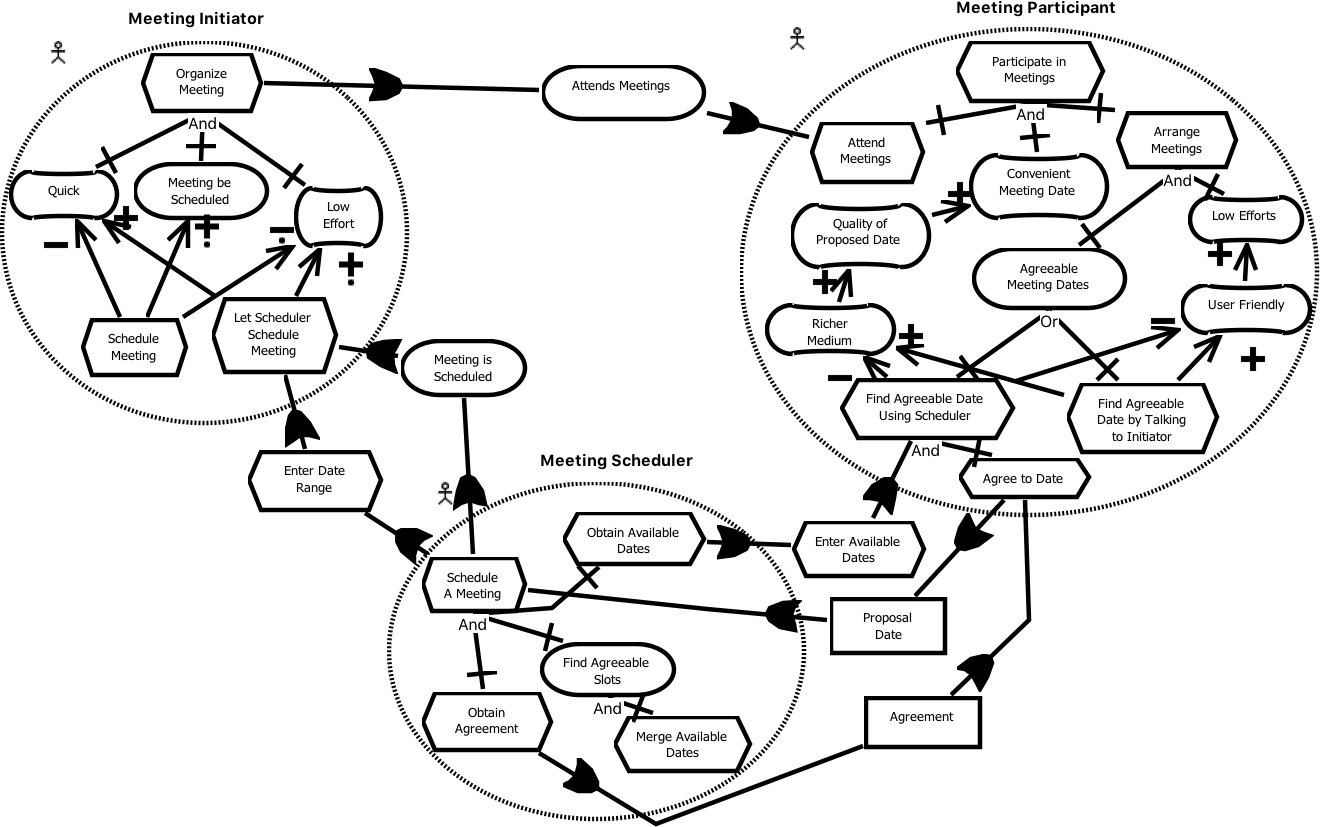
\includegraphics[scale=0.35]{img/SchedulerModel}
\caption{GRL Model for Online Meeting Scheduler}
\label{fig:SchedulerModel}
\end{figure*}

Different links connect the elements in a GRL model. AND, IOR, and XOR decomposition links (
\includegraphics[scale=1]{img/decomposition}) allow an element to be decomposed into sub-elements. In Figure~\ref{fig:SchedulerModel}, the task \textsf{Participate in Meetings} is AND-decomposed to the tasks \textsf{Attend Meetings} and \textsf{Arrange Meetings} as well as the softgoal \textsf{Convenient Meeting Date}. Contribution links (
\includegraphics[scale=1]{img/contribution}) indicate desired impacts of one element on another element. A contribution link has a qualitative contribution type or a quantitative contribution. Softgoal \textsf{User Friendly} has \textsf{some positive} qualitative contribution to the softgoal \textsf{Low Efforts}. Dependency links (
\includegraphics[scale=1]{img/dependency}) model relationships between actors. For example, actor \textsf{Meeting Scheduler} depends on the actor \textsf{Meeting Participant} to \textsf{Agree to Date} via the resource \textsf{Proposal Dates} to fulfill its task \textsf{Schedule a Meeting}.

GRL is based on $i*$~\cite{Yu:1997:TMR:827255.827807} and the NFR Framework~\cite{chung2012non}, but it is not as restrictive as $i*$. Intentional elements and links can be more freely combined, the notion of agents is replaced with the more general notion of actors, i.e., stakeholders, and a task does not necessarily have to be an activity performed by an actor, but may also describe properties of a solution.

\todo{Floris}{Sepideh}{can you haver a look at the motivation for using GRL (below)? It used to be a separate section but I think it fits best here, have a look at what we need. I agree that we can mention jUCMNav but not use it as motivation since we will use online tool.}

GRL is an international standard with well defined syntax and semantics. This allows us to combine the theory of formal argumentation with GRL precisely, hereby satisfying requirement 3 as described in the introduction. Moreover, GRL has an open source tool called jUCMNav, which simplifies an implementation. Since implementation is a key concern for us, the extensive tool support is a strong argument in favor of GRL.  

According to Amyot et al.~\cite{amyot2009lightweight}, GRL has several benefits over other existing goal modeling languages, such as integration with a scenario notation (UCM), support for both qualitative and quantitative attributes (for contributions levels and satisfaction levels), there is a clear separation of GRL model elements from their graphical representation, and it provides support for providing a scalable and consistent representation of multiple views/diagrams of the same goal model (see~\cite[Ch.2]{Ghanavati2013} for an more details). Finally, URN and jUCMNav provide traceability links between concepts and instances of goal modeling and behavioral design models. This traceability enables direct impact analysis of goal changes on a design and vice versa. This traceability feature seems to be a good fit with our current research: We aim to add traceability links between intentional elements and their underlying arguments. \todo{Sepideh}{Sepideh}{I need to improve: GRL has has the capability to be extended via profile, metadata and rules, and due to this capability, it has been extended to many domain. This feature also helps us to apply our argumentation to other domain such as compliance or enterprise architecture. }


\subsubsection{Online Meeting Scheduler Example}
\label{sect:background:casestudy}

In this paper, we use the classic example of an online meeting scheduler that has been used in the literature~\cite{}, ~\cite{}, ~\cite{} several times. The meeting scheduler has been modeled with Tropos~\cite{} and $i*$. We remodel this example with GRL in jUCMNav for the purpose of our framework. 

The meeting scheduler system has three actors, \textbf{Meeting Initiator}, \textbf{Meeting Scheduler} and \textbf{Meeting Participant}. The \textbf{Meeting Scheduler} has a goal that for every meeting request, it has to try to find the best time and location in a way that most of the intended participants (i.e. \textbf{Meeting Participant}) can attend the meeting. The \textbf{Meeting Initiator} organizes the meetings by asking the participants to give their availability for a range of dates and time as well as the dates that they are not available. Based on these information, the \textbf{Meeting Scheduler} needs to pick a date/time and a location from the available dates/times given by the participants in a way that the most number of participants can attend. Participants should then accept or reject the event. 

The GRL model in Figure~\ref{fig:SchedulerModel} shows the softgoals, goals, tasks and the relationship between the different intentional elements in the model. However, the rationales and arguments behind certain intentional elements have not been discussed or illustrated in the GRL model. Some of the questions that might be interesting to know about are the following:

\todo{Sepideh}{Marc}{I think you can add some more or remove/modify some of these based on your needs in the future sections}
\begin{itemize}
	\item Why are only the two softgoals \textbf{Quick} and \textbf{Low effort} selected for the task \textbf{Organize Meeting}? Why is, for example, a goal \textbf{Selecting the most convenient time} not included in the analysis for the actor \textbf{Meeting Initiator}?
	\item What does \textbf{Quality of Proposed Date} mean?
	\item How can one decide if the quality is low or high? Who is in charge? \todo{Floris}{Sepideh}{do you mean the \textbf{Quality of Proposed Date}? Or quality of the GRL diagram?}
	\item Does the meeting initiator use an email to inform the meeting participants to enter their availabilities? 
	\item Does the meeting scheduler uses an online calendar to obtain the available dates or an online website?
	\item How much time do the participants have to enter their availabilities? Is that important? Do they get a reminder from either the initiator or the scheduler? Is the reminder sent via an email? 
	\item What does \textbf{Richer Medium} mean? 
\end{itemize}

\todo[resolved]{Sepideh}{all}{We need to further improve this part}
\todo{Marc}{all}{Improved this part, what do you think?}
These are the type of the questions that we cannot answer just by looking at the GRL models. The model in figure~\ref{fig:SchedulerModel} does not contain such information, such as elements or actions that have been discussed, but did not end up in the final model, discussions that led up to the formation of an element (for instance, by various clarification steps), or alternatives that have been considered for the relationships. In order to address this shortcoming, we use Argument Schemes for Goal Modeling (GMAS). GMAS can help us decide what intentional elements should remain in GRL and what new ones to be added or deleted, provide rationale behind the design decisions and the relationships between the links. 

\subsection{Argument Scheme for Practical Reasoning (PRAS)}
\label{sect:background:pras}

Reasoning about which goals to pursue and actions to take is often referred to as \emph{practical reasoning}, and has been studied extensively in philosophy (e.g. \cite{Raz1978-RAZPR,walton1990}) and Artificial Intelligence \cite{Bratman1987,atkinson2007}. One approach is to capture practical reasoning in terms of arguments schemes and critical questions~\cite{walton1990}. The idea is that an instantiation of such a scheme gives a presumptive argument in favor of, for example, taking an action. This argument can then be tested by posing critical questions about, for instance, whether the action is possible given the situation, and a negative answer to such a question leads to a counterargument to the original presumptive argument for the action. 

A formal approach to persuasive and deliberative reasoning about goals and actions has been presented by Atkinson et al.~\cite{atkinson2007}, who define the Practical Reasoning Argument Scheme (PRAS). PRAS follows the following basic argument structure. 
\begin{equation}
\label{eq:eq1}
  \begin{aligned}
 \qquad&\text{I have goal } G&\\
&\text{Doing action }A \text{ will realize goal }G&\\
&\text{Which will promote value }V&\\
&\text{\emph{Therefore} I should do action }A.&
  \end{aligned}
\end{equation}

So, for example, we can say that 
\begin{itemize}
\item[] \textbf{Find agreeable meeting date} is a goal,
\item[] \textbf{Find agreeable date by talking to initiator} will realize the goal \textbf{(Find) agreeable meeting date},
\item[] Which will promote the value \textbf{User friendliness}
\item[] \textit{Therefore} 
\item[] We should perform action \textbf{Find agreeable date by talking to initiator}
\end{itemize}

Practical reasoning is defeasible, in that conclusions which are at one point acceptable can later be rejected because of new information. Atkinson \emph{et al.}~\cite{atkinson2007} define a set of critical questions that point to typical ways in which a practical argument can be criticized by, for example, questioning the validity of the elements in the scheme or the connections between the elements. Some examples of critical questions are as follows.

\begin{enumerate}
\item Will the action bring about the desired goal?
%\item Does the goal promote the value stated?
\item Are there alternative ways of realizing the same goal?
\item Are there alternative ways of promoting the same value?
%\item Does doing the action have a side effect which demotes the value?
\item Does doing the action have a side effect which demotes some other value?
\item Does doing the action promote some other value?
%\item Does doing the action preclude some other action which would promote some other value?
\item Is the action possible?
\item Can the desired goal be realized?
\item Is the value indeed a legitimate value?
\end{enumerate}

These critical questions can point to new arguments that might counter the original argument. Take, for example, critical question 8. If, for example, there is evidence that schedulers do not care about user friendliness we have a counterargument to the above argument, `evidence shows that \textsf{user friendliness} is not a legitimate value'. Another way to counter an argument for an action is to suggest an alternative action that realizes the same goal (question 2) or an alternative goal that promotes the same value (question 3). For example, we can argue that \textbf{Find agreeable date using scheduler} also realizes the goal \textbf{Find agreeable meeting date}, which gives us a counterargument to the original argument -- to find a date by talking to the initiator -- that also follows PRAS. 

In argumentation, counterarguments are said to \emph{attack} the original arguments (and sometimes vice versa). In the work of Atkinson et al.~\cite{atkinson2007}, arguments and their attacks are captured as an \emph{argumentation framework} of arguments and attack relations as introduced by Dung~\cite{Dung1995}\footnote{Full definitions of Dung's~\cite{Dung1995} frameworks and semantics will be given in section \ref{sect:gmas}. In this section, we will briefly discuss the intuitions behind these semantics.}. Figure \ref{fig:pras:example1} shows an argumentation framework with three arguments from the above example: the argument for \textbf{Find agreeable date by talking to initiator} (A1), the argument for \textbf{Find agreeable date using scheduler} (A3), and the argument that \textbf{User friendliness} is not a legitimate value (A2). The two alternative PRAS instantiations are A1 and A3. These arguments mutually attack each other, as \textbf{Find agreeable date by talking to initiator}  and \textbf{Find agreeable date using scheduler} are considered to be mutually exclusive. Argument A2 attacks A1, as it questions the legitimacy of the value \textbf{User friendliness}. 

\begin{figure}[ht]
\centering
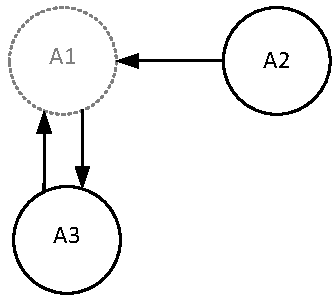
\includegraphics[scale=0.8]{img/Fig1}
\caption{Argumentation framework}
\label{fig:pras:example}
\end{figure}

Given an argumentation framework, the acceptability of arguments can be determined according to the appropriate argumentation semantics. The intuition is that an argument is acceptable if it is \emph{undefeated}, that is, any argument that attacks it, is itself defeated. Take, for example, the argumentation framework in Figure~\ref{fig:pras:example}. Argument A2 is undefeated because it has no attackers. This makes A1 defeated, because one of its attackers, A2, is undefeated. A3 is then also undefeated, since its only attacker, A1, is defeated by A2. Thus, the set of undefeated (justified) arguments given the argumentation framework in Figure~\ref{fig:pras:example} is $\{$A2, A3$\}$. 

In some cases, it is more difficult to determine whether or not an argument is defeated. Take, for example, the argumentation framework with just A1 and A3: they attack each other, they are alternatives and without any explicit preference, it is impossible to choose between the two. It is, however, possible to include explicit preferences between arguments when determining argument acceptability \cite{amgoud2002reasoning}. Take, for example, A1 and A3. If we say that we prefer the action \textbf{Find agreeable date by talking to initiator} (A1) over the action \textbf{Find agreeable date using scheduler} (A3), we remove the attack from A1 to A3 (Figure~\ref{fig:pras:example2}, left). This makes A1 the only undefeated argument, whereas A3 is now defeated. It is also possible to give explicit arguments for preferences \cite{modgil2009}. These arguments are then essentially attacks on attacks. For example, say we prefer A1 over A3 because `the \textbf{Meeting participant} does not like working with a scheduler' (A4). This can be rendered as a separate argument that attacks the attack from A3 to A1 (Figure~\ref{fig:pras:example2}, right), removing this attack and making $\{$A1, A4$\}$ the undefeated justified set of arguments.

\begin{figure}[ht]
\centering
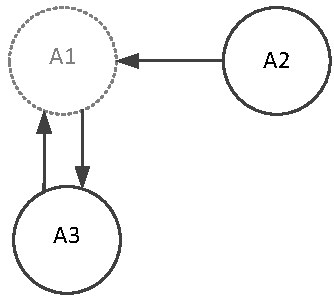
\includegraphics[scale=0.8]{img/Fig2}
\caption{Preferences between arguments}
\label{fig:pras:example2}
\end{figure}  

\subsubsection{Practical Argumentation and Goal Modeling}
\label{sect:background:pras:motivation}

Practical reasoning in the PRAS framework as described above provides a formally sound framework for defeasible reasoning about goals and actions that adheres to the acceptability semantics of Dung~\cite{Dung1995} and its various extensions \cite{amgoud2002reasoning,modgil2009}. The usefulness of PRAS for the analysis of practical reasoning situations has been shown in different areas such as e-democracy~\cite{cartwright2009IS}, law~\cite{atkinson2005legal}, planning \cite{medellin2013planning} and choosing between safety critical actions \cite{tolchinsky2012deliberation}. The question in this paper is how PRAS can be adopted for use in goal modeling, so that we can capture the discussions between stakeholders that build a goal model as formal argumentation, thus adding a new evaluation technique for goal models that allows us to assess the \emph{acceptability} of elements of a goal model (as opposed to the \emph{satisfiability} \cite{}). 

PRAS (actions, goals, values) and GRL (tasks, goals, softgoals) have some obvious similarities, and in previous work \cite{vanzee-etal:renext2015,vanZee-etal:er2016,vanZee-etal:comma2016} we presented arguments based on PRAS of the form ``G is a goal, Action A realizes G \emph{Therefore} perform action A'' (see Figure~\ref{fig:pras:example3}, left, where the arrow denotes an inference step). Such arguments, which can be constructed using the online OVA tool\footnote{\url{http://ova.arg-tech.org/}}, can be combined with further arguments providing, for example, expert opinions about the practical reasoning elements (Figure~\ref{fig:pras:example3}, left).

\begin{figure}[ht]
\centering
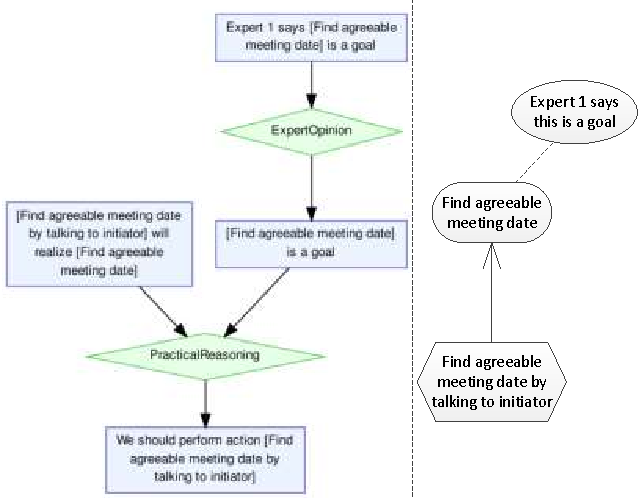
\includegraphics[width=\columnwidth]{img/Fig3}
\caption{Structured argument based on PRAS (left) and the corresponding GRL diagram (right)}
\label{fig:pras:example3}
\end{figure}  

Arguments built in OVA can automatically be translated to GRL diagrams using further online tooling\footnote{\url{https://github.com/RationalArchitecture/RationalGRL}} \cite{vanZee-etal:comma2016}. This translation takes the elements of the arguments and directly translates this to GRL elements. Tasks/actions, goals and softgoals/values can be directly translated from the arguments to the GRL diagrams, as can realization statements. Elements of arguments that have nothing to do with goal modelling (e.g. the expert opinion premise in Figure~\ref{fig:pras:example3}) can be included in the GRL diagram as \emph{beliefs}. Finally, attacks between arguments are captured as negative contribution links. Take, for example, \todo{example}. A very similar approach to argumentation and goal models had already been taken by Jureta et al.~\cite{Jureta:RE2008} who proposed a formal argumentation model that can be used to justify goal-modelling decisions. This argumentation model, while not explicitly based on a practical reasoning scheme, is essentially the same as our previous argumentation model based on PRAS: a formal model of structured arguments with goals as premises and tasks as conclusions, and a translation function of these arguments to goal diagrams. 

The core problem of the use of argumentation in the above-mentioned work \cite{Jureta:RE2008,vanzee-etal:renext2015,vanZee-etal:er2016}, is that it focuses mainly on structured arguments, which are then directly translated to goal models as in Figure~\ref{fig:pras:example3}. The question is what the added value of this exercise is. Firstly, the arguments and goal models contain many of the same elements. The idea is that arguments show the rationales behind goal models and the alternative or possibly conflicting views that were lost in the goal-modeling process. But GRL already contains a \emph{belief} element that allow one to provide beliefs underlying a goal model, an \emph{XOR decomposition} link that allows for modeling of alternative ways to realize goals, and \emph{negative contribution} links for capturing conflicting goals. 

The point is that argumentation models are not needed to precisely render goals, tasks, beliefs and the relations between them, as GRL is already perfectly suited for this. Rather, argumentation should guide the goal modelling \emph{process}. Instead of static, formal argument trees, we need a dynamic argumentation process in which goals and tasks are critically analysed and which captures the dialectical nature of justification. Jureta et al.~\cite{Jureta:RE2008} take a step towards such a process by defining a high-level decision process that organizes argumentation and clarification techniques in relation to goal modelling. However, the argumentation techniques in this process are focused on building precisely the type of arguments that we argue are redundant next to GRL diagrams, namely structured arguments like in Figure~\ref{fig:pras:example3} which can be translated more or less directly to goal models. The decision process itself is never formally defined, and how to go from a discussion on goals and tasks to a goal model remains largely implicit. 

What is needed is a formal framework that captures the discussions about goal models, and allows for (semi-)automated construction of goal models given this discussion. In section XX, we argue that a combination of Atkinson et al.'s~\cite{atkinson2007} critical questions and the dialectical semantics as formally captured by Dung's work \cite{Dung1995} are ideally suited to provide such a formal, dynamic framework.  

\section{Preview of the Framework}
\label{sect:preview}

\todo{Marc}{Marc}{Give an example showing how our framework works without the technical details.}

\section{Argument Schemes for Goal Modeling (GMAS): First Iteration}
\label{sect:gmas}

In this section we develop an initial set of argument schemes and critical questions for goal modeling, based by the argument scheme for practical reasoning as described in the previous section. In the next section, we validate and improve this list by annotating arguments found in transcripts of discussions about an information system.

\begin{table*}[h]
\centering
\begin{tabular}{|l|l|l|l|l|}
\hline
\multicolumn{2}{|c|}{\textbf{Argument scheme}} & \multicolumn{2}{c|}{\textbf{Critical Questions}}\\
\hline
AS0 & Actor $a$ is relevant & CQ0 &Is the actor relevant?\\
\hline
AS1 & Actor $a$ has resource $R$ & CQ1 &Is the resource available?\\
\hline
AS2 & Actor $a$ can perform task $T$ & CQ2 &Is the task possible?\\
\hline
AS3 & Actor $a$ has goal $G$ & CQ3 & Can the desired goal be realized?\\
\hline
AS4 & Actor $a$ has softgoal $S$ & CQ4 & Is the softgoal a legitimate softgoal?\\
\hline
\hline
AS5 & Task $T$ contributes to goal $G$ & CQ5a & Does the task contribute to the desired goal?\\
& & CQ5b & Are there alternative ways of realizing the same goal?\\
\hline
AS6 & Task $T$ contributes to softgoal $S$& CQ6a & Does the task contribute to the softgoal?\\
&& CQ6b & Are there alternative ways of contributing to the same softgoal? \\
&& CQ6c & Does the task have a side effect which contribute negatively to some other softgoal?\\
&& CQ6d & Does the task contribute to some other softgoal?\\
\hline
AS7 & Goal $G$ contributes to softgoal $S$ & CQ7a & Does the goal contribute to the softgoal?\\
&& CQ7b & Does the goal contribute to some other softgoal?\\
\hline
AS8 & Resource $R$ contributes to task $T$ & CQ8 & Is the resource required in order to perform the task?\\
\hline
AS9 & Actor $a$ depends on actor $b$ & CQ9 & Does the actor depend on any actors?\\
\hline
\end{tabular}
\caption{Initial list of argument schemes and critical questions for GRL elements (AS0-AS4) and relationships (AS5-AS16).}
\label{table:argument-schemes}
\end{table*}

\subsection{Argument schemes and critical questions}

Where PRAS consists of the single argument scheme PAS, our approach is to split this into a family of argument schemes, such that each separate argument scheme can be applied to a specific part of a goal model. Similar to PRAS, someone who does not accept the presumptive argument may challenge it by applying critical questions. We have modified Atkinson et al.'s original 16 questions associated with the scheme \cite{atkinson2006argumentation} by removing those questioning elements not part of GRL (\emph{circumstances}), adding questions for additional elements GRL (\emph{resources}), and renaming concepts and relationships (e.g., the \emph{promotes} relationship).

The initial list We developed a total of 10 argument schemes and 18 critical questions, which are shown in table~\ref{table:argument-schemes}. Argument schemes AS0-AS4 can be instantiated for individual GRL elements, and each have a single critical question. CQ2-CQ4 are critical questions by Atkinson rephrased using the GRL terminology, while CQ1 is added in order to question a resource element, which does not appear in PRAS. AS5-AS9 are argument schemes for various GRL relationships between elements. As we mentioned before, this list is not meant to be exhaustive, since GRL does not put restrictions on any of relationships, so in theory any type of element can be combined with any type of elements, using any relationship. Here we merely use the critical questions developed by Atkinson et al.
 
Answering a critical question results in the creation of a new argument, which may or may not attack the original arguments, depending on which question is answered. For instance, answering CQ1 with ``no'' results in a new argument attacking the argument that actor $a$ has resource $R$ available. In contrary, answering CQ5b with ``yes'' does not result in an attack on the original argument, but creates a new argument stating that some other task realizes the goal as well. We will return to this issue in more detail in the next section. In the current section, we restrict our analysis to the development of appropriate argument schemes and critical questions.

\section{GMAS: Second iteration}
\label{sect:gmas:2}

The argument schemes and critical questions of Table~\ref{table:argument-schemes} are based on the theoretical work by Atkinson, and our own observations about the differences with GRL. However, it is unclear whether this list is exhaustive, or even whether the schemes and questions are actually used in practice. In order to evaluate this, we annotate transcripts of discussions between students with the arguments occurring in them, and analyze the results in order to refine our list.

\subsection{Empirical evaluation with transcripts}

The transcripts we used are created as part of two master theses on improving design reasoning~\cite{masterthesis1,masterthesis2}.

\paragraph{Subjects} The subjects for the case study are three teams of Master students from the University of Utrecht, following a Software Architecture course. Two teams consist of three students, and one team consists of two students.

\paragraph{Experimental Setup} The assignment used for the experiments is to design a traffic simulator. Designers are provided a problem description, requirements, and a description of the desired outcomes. The original version of the problem descrption~\cite{UCIworkshop} is well known in the field of design reasoning since it has been used in a workshop\footnote{\url{http://www.ics.uci.edu/design-workshop/}}, and transcripts of this workshop have been analyzed in detail~\cite{Petre:2013:SDA:2535028}. Although the concepts of traffic lights, lanes, and intersections are common and appear to be simple, building a traffic simulator to represent these relationships and events in real time turns out to be challenging. Participants were asked to use a think-aloud method during the design session. For the student groups the assignment was slightly adjusted to include several viewpoints as end products in order to conform to the course material~\cite{Bass:2012:SAP:2392670}. The final problem descriptions can be found in Appendix A of Schriek's master thesis~\cite{masterthesis1}. All groups were instructed to apply the functional architecture method (FAM), focusing on developing the Context, the Functional, and the Informational viewpoint of the traffic simulator software. The students had two hours for the tasks, and the transcripts document the entire discussion. The details of the transcripts are shown in table~\ref{table:transcripts:info}.

\begin{table}[ht]
\centering
\begin{tabular}{|l|l|l|l|}
\hline
& transcript $t_1$ & transcript $t_2$ & transcript $t_3$\\
\hline
participants & 2 & 3 & 3\\
\hline
duration & 1h34m52s & 1h13m39s & 1h17m20s\\
\hline
\end{tabular}
\caption{Number of participants and duration of the transcripts.}
\label{table:transcripts:info}
\end{table}

\paragraph{Annotation method} We annotated transcripts with the arguments and critical questions of table~\ref{table:argument-schemes}. If we found arguments or critical questions that did not appear in the list, we added them and counted them as well. Most of the occurrences were not literally found back, but had to be inferred from the context. For instance, if a participant questions an argument with a statement such as ``I don't know about that'', then we interpret this as a critical question.

It is generally known in the argumentation literature that it can be very difficult to annotate arguments correctly.\todo{Marc}{Floris}{add citation} Arguments are often imprecise, lack conclusion, and may be supported by non verbal communication that is not captured in the transcripts. Still, since research on argument extraction in the requirement engineering domains is in its infancy, we believe that our evaluation is useful by itself. Furthermore, our annotation is openly available\footnote{\todo{Marc}{Marc}{provide url}}, we provide parts of our annotation in Appendix~\ref{sect:transcripts:excerpts}, and most of the examples from this article come from the transcripts. In this way, we aim to make our annotation process as transparent as possible.

\subsubsection{Results}

Some examples of annotation can be found in appendix~\ref{sect:transcripts:excerpts}. We found a total of 120 instantiations of the existing argument schemes AS0-AS9 in the transcripts. The most used argument scheme was AS2: ``Actor $A$ has task $T$'', but each argument scheme has been found back in the transcripts at least twice (table~\ref{table:transcripts:results:argumentschemes}). Examples of argument schemes are AS1, an argument for a resource (table~\ref{table:transcript:as1-as8}); AS2, an argument for a task (tables~\ref{table:transcript:as2-cq_star_1-cq2},~\ref{table:transcript:as2-cq_star_2}, and~\ref{table:transcript:as2-as10}); AS4, an argument for a softgoal, AS5, an argument for a goal, AS7, an argument for a contribution from goal to softgoal (table~\ref{table:transcript:as4-as5-as7}); and AS8, an argument for a contribution from resource to task (table~\ref{table:transcript:as1-as8}). 

Of our critical questions, we annotated 9 instantiations. Example of critical questions are CQ0, questioning the relevance of an actor (table~\ref{table:transcript:as0-cq0}) and CQ2, questioning the possibility of a task (table~\ref{table:transcript:as2-cq_star_1-cq2}).

\begin{table}[ht]
\centering
\begin{tabular}{|l|l|l|l|>{\bfseries}l|}
\hline
\textbf{Argument Schemes} & $t_1$ & $t_2$ & $t_3$ & \textbf{total}\\
\hline 
AS0: Actor & 2 & 2 & 5 & 9\\
\hline
AS1: Resource & 2 & 4 & 5 & 11\\
\hline
AS2: Task/action & 20 & 21 & 17 & 58\\
\hline
AS3: Goal & 0 & 2 & 2 & 4\\
\hline
AS4: Softgoal & 3 & 4 & 2 & 9\\
\hline
AS5: Goal decomposes into Task & 4 &0& 4 & 8\\
\hline
AS6: Task contributes to softgoal & 6 & 2 &0& 8\\
\hline
AS7: Goal contributes to softgoal &0& 1 & 1 & 2\\
\hline
AS8: Resource contributes to task & 0 & 4 & 3 & 7\\
\hline
AS9: Actor depends on actor &0& 1 & 3 & 4\\
\hline
\hline
\textbf{TOTAL} & 37& 41 & 42 & 120\\
\hline
\end{tabular}
\caption{Number of occurrences of AS0-AS9 in the transcripts.}
\label{table:transcripts:results:argumentschemes}

\begin{tabular}{|l|l|l|l|>{\bfseries}l|}
\hline
\textbf{Critical questions} & $t_1$ & $t_2$ & $t_3$ & \textbf{total}\\
\hline 			
CQ2: Task is possible? & 2 & 2 & 1 & 5\\
\hline		
CQ5a: Does the task contribute to the the goal? & 0 & 1 & 0 & 1\\
\hline
CQ5b: Alternative ways to realize the same goal? & 1 & 0 & 0 & 1\\
\hline
CQ6b: Task has negative side effects? & 2 & 0 & 0 & 2\\
\hline
\hline
\textbf{TOTAL} & 5 & 2 & 1 & 9\\
\hline
\end{tabular}
\caption{Number of occurrences of critical questions CQ0-CQ9 in the transcripts. Critical questions not appearing in this table were not found back in the transcripts.}
\label{table:transcripts:results:criticalquestions}
\end{table}

Additionally, we identified 85 statements that did not fit our existing argument schemes and critical questions, leading to 2 new argument schemes (39 occurrences) and 8 new critical questions (29 occurrences). The new argument schemes and critical questions are shown in table~\ref{table:transcripts:results:new}. 

\subsubsection{Analysis}

The analysis of the results of our empirical evaluation consists of three parts. First, we analyze the argument schemes, then the critical questions, and finally we analyze the effect of posing a new argument.

\paragraph{Analysis of the argument schemes}
The difference between the initial list of argument schemes and those found back in the transcripts is quite small. We found it surprising that we were able to find back all the schemes in the transcript at least twice, even more since the topic of discussion wasn't goal models, but more generally the architecture of an information system. This gives us an indication that these argument schemes are able to capture arguments used in those type of discussions to some extent. However, we also found the following additional argument schemes:
\begin{itemize}
\item
\emph{AS10: Task decomposes into task.} While our initial list of argument schemes contains a scheme to decompose goals into tasks (AS5), it does not contain one for task decomposition. We found that are large part of the discussions were focused around the tasks that the information system should provide. In the first phase of the discussion, participants often listed a number of tasks the information system should provide (table~\ref{table:transcript:as2-cq_star_1-cq2}), which were then later refined through task decomposition (table~\ref{table:transcript:as2-as10}).
\item 
\emph{AS11: Task contributes negatively to softgoal.}  We found that participants occasionally discuss negative contributions as well (table~\ref{table:transcript:as11}).
\end{itemize}
More generally, we observed that our initial list is rather limited, which is a consequence of the fact that it is derived from PRAS. Since PRAS only considers very specific types of relationships, we are not able to capture many other relationships existing in GRL. GRL has four types of intentional elements (softgoal, goal, task, resource) and four types of relationships (positive contribution, negative contribution\footnote{In fact, a contribution can be any integer in the domain [-100,100], but for the sake of simplicity we only consider two kinds of contributions here.}, dependency, decomposition), allowing theoretically $4^3=64$ different types of argument schemes, of which we currently only consider 5. Our analysis shows that many of these schemes are not often used, but we should at least add the possibility for task decomposition (AS10) and negative contribution (AS11).

\begin{table*}[ht]
\centering
\begin{tabular}{|l|l|l|l|>{\bfseries}l|}
\hline
\textbf{New annotation} & $t_1$ & $t_2$ & $t_3$ & \textbf{total}\\
\hline
AS10: Task decomposes into task & 11 & 14 & 11 & 36\\
\hline
- CQ10a: Does the task decompose into other tasks? & 1 &2 &0&3\\
\hline
- CQ10b: Is the decomposition correct (AND/OR/XOR)? &1 &0& 1 &2\\
\hline
AS11: Task contributes negatively to softgoal&2&1	&0&3\\
\hline
\hline
TI: Topic introduction & 5 & 3 & 7 &15\\
\hline
REM: Removing useless/irrelevant/redundant element & 2 & 3 & 2 &7\\
\hline
CLAR: Clarifying an element &3 &10 & 3 & 16\\
\hline
GEN: Generic counterargument	& 0& 2 & 2 & 4\\
\hline
\textbf{TOTAL}&24&34&25&87\\
\hline
\end{tabular}
\caption{Number of occurrences of new argument schemes and critical questions in the transcripts.}
\label{table:transcripts:results:new}
\end{table*}

\paragraph{Analysis of the critical questions} The difference between the initial list of critical questions and those we found back in the transcripts is much larger than for the critical questions. On the one hand, we found back few of the critical questions we initially proposed. However, this does not mean that they weren't implicitly used in the minds of the participants. If a participants makes an argument for a contribution from a task to a softgoal, it may very well be that she was asking herself the question ``Does the task contribute to some other softgoal?''. However, many of these critical questions are not mentioned explicitly. If we assume this explanation is at least partially correct, then this would mean that critical questions may still play a role when formalizing the discussions leading up to a goal model, and it would be limiting to leave them out of our framework. In the context of tool support, we feel that having these critical questions available may stimulate discussions.

On the other hand, we found back relatively many new critical questions that were not on our initial list. We found back two critical questions for the new argument schemes AS10:
\begin{itemize}
\item \emph{CQ11a: Does the task decompose into other tasks?} (table~\ref{table:transcript:cq:task_decomp}).
\item \emph{CQ11b: Is the decomposition correct? (AND/OR/XOR)} The initial list of critical questions does not distinguish between the type of decomposition that may occur. However, we found that this is sometimes discussed by participants (table~\ref{table:transcript:cq11b}).
\end{itemize}
Moreover, we found four types arguments that we could not classify as an instantiation of an argument scheme or a critical question:
\begin{itemize}
\item \emph{Topic introduction.} Before posing arguments, participants often proposed to discuss a certain topic, for instance by stating ``we have to determine who the users of the system are gonna be'' (table~\ref{table:transcript:as-star})..
\item \emph{Removing useless/irrelevant/redundant element} We found this critical question especially in relation with tasks (table~\ref{table:transcript:as2-cq_star_1-cq2}).
\item \emph{Clarifying an element} Given the large body of literature on clarification \todo{Marc}{Marc}{add citations}, it is not surprising that we found this type of argument relatively often. We do not aim to provide a detailed analysis of the different types of clarification techniques in this article, but we merely want to be able to capture an argument clarifying a previous argument in a course grained way. Such an analysis in the context of argumentation and requirement engineering can be found elsewhere~\cite{Jureta:RE2008}. See table~\ref{table:transcript:as2-cq_star_2} for an example of a clarification argument.

\item \emph{CQ: Generic counterargument.} Participants occasionally posed counterarguments against arguments or critical questions as well, which we could not classify further (table~\ref{table:transcript:as0-cq0-cq_counterarg}).
\end{itemize}

\paragraph{Analysis of the effect of a new argument} When a new argument is put forward, this can have varying effects on the previous arguments. For instance, in the excerpt of table~\ref{table:transcript:as0-cq0}, the answer to the critical questions results in an argument attacking the original argument for actor ``Development team'', which ensures that ``Development team'' is no longer considered to be a relevant actor of the system. In table~\ref{table:transcript:as2-cq_star_2}, answering the critical question also results in an attack on the original argument for task ``car influx'', but at the same time also generates a new argument for a more specific task ``control car influx per road''. In general, we found the following four operations that may be associated with the arguments:

\todo{Marc}{Marc/Floris}{Say that an argument is attacked in different ways and we have to distinguish this}
\begin{itemize}
\item \emph{INTRO: Introduce new element/link.} This operation does not attack anything, but generates new elements. Examples are CQ5b, CQ6c, and \emph{Topic introduction}.
\item \emph{DISABLE: Disable element/link.} This operation generates an attack on an element or link but does not replace it with anything. Examples are CQ0-CQ4, CQ5a, and \emph{Clarifying an element}.
\item \emph{REPLACE: Replace element/link.} This operation replaces the description of the intentional element, or it replaces the type of link (e.g., from positive contribution to negative contribution, or from AND-decomposition or OR-decomposition). An example is \emph{Clarifying an element}.
\item \emph{GENERIC: Generic counterargument.} This operation simply directly attacks an argument. It is different from DISABLE in the sense that it only attacks one argument directly, while DISABLE attacks an argument for an element/link, and all possible previous replacements for it. We explain this in more detail in the next section where we introduce our algorithms.
\end{itemize}

\subsection{Final argument schemes and critical questions}

Our final set of argument schemes are AS0-AS9 (table~\ref{table:argument-schemes} and AS10-AS11 (table~\ref{table:transcripts:results:new}, and the final set of critical questions are CQ0-C9 (table~\ref{table:argument-schemes} and CQ10 (table~\ref{table:transcripts:results:new}. Additionally, we add the four arguments TI, REM, CLAR, and GEN (table~\ref{table:transcripts:results:new}.

In the end of the previous section we distinguished four operations (REPLACE, DISABLE, INTRO, and GENERIC) that can be applied when instantiating an argument scheme or answering a critical question. In table~\ref{table:operation-mappings} we provide a mapping form our argument schemes, critical questions, and additional arguments to these four operations. In the next section, we formalize these operations as algorithms.

\begin{table}[ht]
\begin{tabular}{|l|l|}
\hline
\textbf{Argument} & \textbf{Operation}\\
\hline
AS0-AS11, CQ5b,CQ6b-d,CQ7b,TI& INTRO\\
\hline
CQ0-CQ4,CQ5a,CQ6a,CQ7a,CQ8,CQ9,REM & DISABLE\\
\hline
CLAR & REPLACE\\
\hline
GEN & GENERIC\\
\hline
\end{tabular}
\caption{Mapping from the final argument schemes AS0-AS11, final critical questions CQ0-CQ10, and additional arguments TI, REM, CLAR, GEN to the operations.}
\label{table:operation-mappings}
\end{table}

\section{The Formal Framework}
\label{sect:formalframework}

We briefly summarize our results so far and our tasks for the current section. In the previous two sections we developed argument schemes and critical questions for goal modeling in two iterations. In section~\ref{sect:gmas} we proposed an initial list, which we derived from PRAS and the elements and relationships used in GRL (table~\ref{table:argument-schemes}). We then validated this set using transcripts in section~\ref{sect:gmas:2}. This resulted in new argument schemes and critical questions, and also in four new types of arguments that we distinguished from argument schemes and critical questions, namely Topic Introduction (TI), Removing redundant elements (REM), Clarifying an element (CLAR), and Generic counterargument (GEN) (table~\ref{table:transcripts:results:new}). We distinguished four types of operations that can be applied when putting forward an argument, namely Introducing a new element (INTRO), Disabling an element (DISABLE), Replacing an element (REPLACE), and adding a Generic Counterargument (GENERIC). In table~\ref{table:operation-mappings} we provided a mapping from our final list of arguments to these operations.

In this section we develop a formal framework for the arguments and operations on them. In the first subsection we develop a formal language for a GRL model, consisting of actors, intentional elements (softgoals, goals, tasks, and resources), and links (decomposition, positive contribution, negative contribution, and dependency) between intentional elements. In the second subsection we then provide formal definitions of all argument schemes, which are simply statements about a goal model. In the third subsection we formalize the critical questions.

\subsection{Formal Language for a GRL Model}

In order to formalize the arguments used when discussing a goal model, we first provide a formal language for a goal model. The arguments are simply statements in using this language.

In our language, each element of a goal model is denoted by a non-negative integer. We distinguish the actors, intentional elements (softgoals, goals, tasks, and resources), the links (decomposition, positive contribution, negative contribution, and dependency) between intentional elements in three separate sets.

\begin{definition}[Elements]
Let $\{i_1,\ldots,i_n\}\subset \mathbb{N}$ denote the set of elements of a goal model.
The actors are denoted by $Actors=\{i_1,\ldots,i_k\}$, the intentional elements are denoted by $IEs=\{i_{k+1},\ldots,i_m\}$, and the relationships are denoted by $Links=\{i_{m+1},\ldots,i_n\}$.
\end{definition}

We formalize the description of an actor or an intentional element with a proposition $name(i,p)$. Note that links do not have a description.

\begin{definition}[Name of IE or Actor]
The name $p$ of a element $i\in IEs\cup Actors$ is denoted by $name(i,p)$.
\end{definition}

All intentional elements are collected in the set $IEs$. In order to distinguish softgoals, goals, tasks, and resources, we use the following definition.

\begin{definition}[Intentional Element]
Given an intentional element $i\in IEs$, if $i$ is a softgoal, goal, task, or resource, then this is respectively denoted by $softgoal(i), goal(i), task(i)$, and $resource(i)$.
\end{definition}

In the same way, we distinguish between the different types of links between IEs using the following definition.

\begin{definition}[Links]
Given a link $i\in Links$, we denote with $contrib(i,src,dest,type)$ a contribution from $src\in IEs$ to $dest\in IEs$, where $type\in\{pos,neg\}$ means a positive resp. negative contribution. We denote with $decomp(i,src,\{dest_1,\ldots,dest_n\},type)$ a decomposition of $src\in IEs$ into $\{dest_1,\dots,dest_n\}\subseteq IEs$, where $type\in\{AND,OR,XOR\}$ means respective an AND, OR, and XOR decomposition. We denote with $dep(i,d_1,d_2,d_3)$ a dependency from $d_1\in IEs$ via $d_2\in IEs$ to $d_3\in IEs$.
\end{definition}

In order to denote that an intentional element or a link belongs to an actor, we use $has$ statements.

\begin{definition}[Elements of an actor]
Given an actor $i\in Actors$ and a element $j\in IEs\cup Links$, we use $has(i,j)$ to denote that element $j$ belongs to actor $j$.
\end{definition}

\todo{Marc}{Marc}{Provide example here}

\subsection{Formalizing the argument schemes}

In order to formalize the argument schemes we first note that an 

\section{The RationalGRL Tool}
\label{sect:implementation}



\section{The RationalGRL Methodology}
\label{sect:methodology}

The methodology we propose in this paper is visualized in figure~\ref{fig:rationalgrl-methodology}. There are two main activities, depicted in grey, namely "goal modeling" and "argumentation". These are two separate activities that are being done in parallel. 

\begin{figure}[ht]
\centering

\includegraphics[scale=0.4]{img/methodology}
\caption{The RationalGRL Methodology}
\label{fig:rationalgrl-methodology}
\end{figure}

\section{Related Work}
\label{sect:relatedwork}

There are several contributions that relate argumentation-based techniques with goal modeling. The contribution most closely related to ours is the work by Jureta \emph{et al.}~\cite{Jureta:RE2008}. This work proposes ``Goal Argumentation Method (GAM)'' to guide argumentation and justification of modeling choices during the construction of goal models. One of the elements of GAM is the translation of formal argument models to goal models (similar to ours). In this sense, our \textsf{RationalGRL} framework can be seen as an instantiation and implementation of  part of the GAM. One of the main contribution of \textsf{RationalGRL} is that it also takes the acceptability of arguments as determined by the argumentation semantics \cite{Dung1995} into account when translating from arguments to goal models.  \textsf{RationalGRL} also provides tool support for argumentation, i.e. Argument Web toolset, to which OVA belongs \cite{bex2013implementing}, and for goal modeling, i.e. jUCMNav~\cite{jUCMNav}. Finally, \textsf{RationalGRL} is based on the practical reasoning approach of \cite{Atkinson2014}, which itself is also a specialization of Dung's~\cite{Dung1995} abstract approach to argumentation. Thus, the specific critical questions and counterarguments based on these critical question proposed by~\cite{Atkinson2014} can easily be incorporated into \textsf{RationalGRL}. 

\textsf{RationalGRL} framework is also closely related to frameworks that aim to provide a design rationale (DR)~\cite{shum2006hypermedia}, an explicit documentation of the reasons behind decisions made when designing a system or artefact. DR looks at issues, options and arguments for and against the various options in the design of, for example, a software system, and provides direct tool support for building and analyzing DR graphs. One of the main improvements of \textsf{RationalGRL} over DR approaches is that \textsf{RationalGRL} incorporates the formal semantics for both argument acceptability and goal satisfiability, which allow for a partly automated evaluation of goals and the rationales for these goals. 

Arguments and requirements engineering approaches have been combined by, among others, Haley \emph{et al.}~\cite{haley2005arguing}, who use structured arguments to capture and validate the rationales for security requirements. However, they do not use goal models, and thus, there is no explicit trace from arguments to goals and tasks. Furthermore, like~\cite{Jureta:RE2008}, the argumentative part of their work does not include formal semantics for determining the acceptability of arguments, and the proposed frameworks are not actually implemented. Murukannaiah \emph{et al.}~\cite{murukannaiah2015resolving} propose Arg-ACH, an approach to capture inconsistencies between stakeholders' beliefs and goals, and resolve goal conflicts using argumentation techniques.

\section{Conclusions and Future Work}
\label{sect:conclusion}

In this paper, we developed and implemented a framework to trace back elements of GRL models to arguments and evidence that derived from the discussions between stakeholders. We created a mapping algorithm from a formal argumentation theory to a goal model, which allows us to compute the evaluation values of the GRL IEs based on the formal semantics of the argumentation theory. 

There are many directions of future work. There are a large number of different semantics for formal argumentation, that lead to different arguments being acceptable or not. It would be very interesting to explore the effect of these semantics on goal models. Jureta \emph{et al.} develop a methodology for clarification to address issues such as ambiguity, overgenerality, synonymy, and vagueness in arguments. Atkinson \emph{et al.}~\cite{atkinson2007} define a formal set of critical questions that point to typical ways in which a practical argument can be criticized. We believe that critical questions are the right way to implement Jureta's methodology, and our framework would benefit from it. In addition, currently, we have not considered the \emph{Update} step of our framework (Figure~\ref{fig:overview}). That is, the translation from goal models to argument diagrams is still missing. The \emph{Update} step helps analysts change parts of the goal model and analyze its impact  on the underlying argument diagram. Finally, the implementation is currently a browser-based mapping from an existing argument diagramming tool to an existing goal modeling tool. By adding an argumentation component to jUCMNav, the development of goal models can be improved significantly. 

\section*{Acknowledgments}
Marc van Zee is funded by the National Research Fund (FNR), Luxembourg, by the Rational Architecture project.

\bibliographystyle{abbrv}
\bibliography{references}

\newpage

\onecolumn
\appendix

\section{Transcripts excerpts}
\label{sect:transcripts:excerpts}

\begin{table}[!htbp]
\centering
\begin{tabular}{|p{20mm}|p{70mm}|p{60mm}|}
\hline
Respondent & Text & Annotation\\
\hline
0:10:55.2 (P1) & Maybe developers &\textbf{[4 actor (AS0)]} Development team\\
\hline
0:11:00.8 (P2) & Development team, I don't know. Because that's- in this context it looks like she's gonna make the software & \textbf{[5 critical question CQ0 for 4]} Is actor "development team" relevant?\newline
\textbf{[6 answer to 5]} No, it looks like the professor will develop the software.\\
\hline
\end{tabular}
\caption{AS0: Actor, CQ0: Relevant actor? (transcript $t_3$)}
\label{table:transcript:as0-cq0}

\begin{tabular}{|p{20mm}|p{70mm}|p{60mm}|}
\hline
Respondent & Text & Annotation\\
\hline
0:19:08.6 (P3) & Should have a link with an outsource program for the statistical distribution [inaudible] & \textbf{[21 resource (AS1)]} Actor System has resource ``Statistics library''\\
\hline
0:35:27.4 (P3) & Maybe before traffic simulation view you can- the outsource package that makes the map	& \textbf{[38 contribution (AS8)]} Resource ``Statistics library'' contributes to task ``Display traffic simulation''\\
\hline
\end{tabular}
\caption{AS1: Resource, AS8: Resource contributes to task (transcript $t_3$)}
\label{table:transcript:as1-as8}

\begin{tabular}{|p{20mm}|p{70mm}|p{60mm}|}
\hline
Respondent & Text & Annotation\\
\hline
0:15:11.2 (P1) & And then, we have a set of actions. Save map, open map, add and remove intersection, roads & \multirow{2}{60mm}{\textbf{[20 task (AS2)]} Student has tasks ``save map'', ``open map'', ``add intersection'', ``add road'', ``add traffic light'', ``remove intersection''}\\
\cline{1-2}
0:15:34.7 (P2) & Yeah, road. Intersection, add traffic lights	&\\
\hline
0:15:42.3 (P1) & Well, all intersection should have traffic lights so it's & \textbf{[21 critical question CQ*1 for 20]} Is the task ``Add traffic light'' useful/redundant? \newline
\textbf{[22 answer to 22]} Not useful, because according to the specification all intersections have traffic lights.\\
\hline
0:15:52.3 (P1) & (..) And on the technical side it's gonna be a real pain to remove one intersection you're gonna have to remove a lot more because there are only four-ways allowed and if you remove one intersection then-& \textbf{[23 critical question CQ2 for 20]} Is the task ``Remove intersection'' possible?\newline
\textbf{[24 answer to 22]} It is going to be very difficult to implement.\\
\hline
\end{tabular}
\caption{AS2: Task, CQ*1: Redundant element, CQ2: impossible task (transcript $t_1$)}
\label{table:transcript:as2-cq_star_1-cq2}

\begin{tabular}{|p{20mm}|p{70mm}|p{60mm}|}
\hline
Respondent & Text & Annotation\\
\hline
0:23:20.4 (P1) & So, sets, yeah, car influx & \textbf{[32 task (AS2)]} Student has task ``car influx''\\
\hline
0:23:41.2 (P2) & (..) If you can only control the set amount of influx from any side of this sort of random distribution, I think that is going to be less interesting than when you can say something like, this road is frequently traveled. (...) So setting it per road, I think is something we want & \textbf{[33 critical question CQ*2 on 36]} Is the task description specific/clear enough? \newline
\textbf{[34 answer to 37]} No, it is not clear where the influx is changing. Change to ``control car influx per road''\\
\hline
\end{tabular}
\caption{AS2: Task, CQ*2: Specify/clarify element (transcript $t_1$)}
\label{table:transcript:as2-cq_star_2}

\begin{tabular}{|p{20mm}|p{50mm}|p{80mm}|}
\hline
Respondent & Text & Annotation\\
\hline
0:14:31.2 (P1) & Let's see- she uses the system in her course to explain her lectures about traffic problem thing & \textbf{[11 softgoal (AS4)]} ``Explain lectures traffic theory'' (Professor)\newline
\textbf{[12 goal (AS5)]} ``Use traffic light system'' (Professor)\newline
\textbf{[13 contribution (AS7)]} ``use traffic light system'' contributes to ``explain lectures traffic theory''\\
\hline
\end{tabular}
\caption{AS4: softgoal, AS5: goal, AS7: contribution (transcript $t_3$)}
\label{table:transcript:as4-as5-as7}

\begin{tabular}{|p{20mm}|p{90mm}|p{40mm}|}
\hline
Respondent & Text & Annotation\\
\hline
0:00:10.2\newline PERSON 1 & 	So, yeah [pause] I would start with something about the context. That we have to determine who the users of the system are gonna be, stakeholders. & \textbf{[1 topic]} What are the actors?\\
\hline
\end{tabular}
\caption{AS*: Topic introduction (transcript $t_1$)}
\label{table:transcript:as-star}
\end{table}

\begin{table}[!htbp]
\centering
\begin{tabular}{|p{20mm}|p{70mm}|p{60mm}|}
\hline
Respondent & Text & Annotation\\
\hline
0:29:59.5 (P3) & (...) a variety of sequences and timing schemes should be allowed.  (...) we would have traffic light behavior gives you, I guess two options then. & \multirow{4}{60mm}{\textbf{[42 task (AS2)]} Student has task ``set sequence scheme''\newline
\textbf{[43 task (AS2)]} Student has task ``set timing scheme'' \newline
\textbf{[44 decomposition (AS10)] }Task ``set traffic light behavior'' XOR-decomposes into ``set sequence scheme'' and ''set timing scheme''}\\
\cline{1-2}
0:30:23.6 (P1) & Sequences and timing schemes &\\
\cline{1-2}
0:30:25.0 (P3) & Sequences and timing schemes. So you can either go for, yeah, sequences-&\\
\cline{1-2}
0:30:30.9 (P1) & Or timing schemes&\\
\hline	
\end{tabular}
\caption{AS2: Task, AS10: Task decomposition (transcript $t_2$)}
\label{table:transcript:as2-as10}

\begin{tabular}{|p{20mm}|p{70mm}|p{60mm}|}
\hline
Respondent & Text & Annotation\\
\hline
0:30:10.3 (P1) & 	Yeah. But this is- is this an OR or an AND? & \multirow{3}{60mm}{\textbf{[26 critical question CQ*0 for 20]} Is the OR-decomposition of ``simulate'' correct?\newline
\textbf{[27 answer to 26]} No, it should be an AND because the system can do both.}\\
\cline{1-2}
0:30:14.3 (P3) &I think it's an OR&\\
\cline{1-2}
0:30:15.4 (P1) & for the data, it's an OR (...) And for the system it's an AND. (...) Static manner or dynamic. But the system can do both&\\
\hline	
\end{tabular}
\caption{CQ11b: Incorrect decomposition (transcript $t_3$)}
\label{table:transcript:cq11b}

\begin{tabular}{|p{20mm}|p{100mm}|p{30mm}|}
\hline
Respondent & Text & Annotation\\
\hline
0:06:29.3 (P2) & So, is that a trade-off. I think so. &\multirow{2}{30mm}{\textbf{[10 negative contribution (AS11)]}  task ``generate cars randomly'' contributes negatively to softgoal ``dynamic simulation''}\\	
\cline{1-2}
0:06:36.0 (P1) & Yeah, performance versus, I don't know, functionality. Like, what you say, cars come out at the end of the map side [are generated randomly] is performance wise and, I don't know, easier to make but it is less functional. Because you can't see traffic flows that easy because, well there's fixed amount of cars so there's not really gonna be jams [the simulation is less dynamic]. Is there around Utrecht always the same amount of cars? &\\
\hline	
\end{tabular}
\caption{AS11: Negative decomposition (transcript $t_1$)}
\label{table:transcript:as11}

\begin{tabular}{|p{20mm}|p{80mm}|p{50mm}|}
\hline
Respondent & Text & Annotation\\
\hline
0:49:05.3 (P3)&So, density, speed and, is there anything else.&\multirow{3}{50mm}{\textbf{[68 critical question for 63c]} Does ``set road characteristics'' decompose into any other tasks?\newline
\textbf{[69 answer to 68]} Yes, type of cars.}\\
\cline{1-2}
0:49:20.1 (P1) & Maybe type of cars&\\	
\cline{1-2}
0:49:22.0 (P3) & Type of cars, because you could have trucks, you could have personal cars. That would be good because-&\\
\hline	
\end{tabular}
\caption{CQ: Does a task decompose into other tasks? (transcript $t_2$)}
\label{table:transcript:cq:task_decomp}

\begin{tabular}{|p{20mm}|p{60mm}|p{70mm}|}
\hline
Respondent & Text & Annotation\\
\hline

0:10:55.2 (P1) & Maybe developers or & \textbf{[4 actor (AS0)]} Development team\\
\hline
0:11:00.8 (P2)&Development team, I don't know. Because that's- in this context it looks like she's gonna make the software&\textbf{[5 critical question CQ0 for 4]} Is actor ``development team'' relevant?\newline
\textbf{[6 answer to 5]} No, it looks like the professor will develop the software.\\
\hline
..&..&..\\
\hline
0:18:13.4 (P2) & I think we can still do developers here. To the system & \multirow{2}{70mm}{\textbf{[16 counter argument for 6]} According to the specification the professor doesn't actually develop the software.}\\
\cline{1-2}
0:18:22.9 (P1)&Yeah, when the system gets stuck they also have to be [inaudible] ok. So development team&\\	
\hline	
\end{tabular}
\caption{AS0: Task, CQ0: Relevant task? CQ: Generic counterargument (transcript $t_2$)}
\label{table:transcript:as0-cq0-cq_counterarg}

\end{table}




\end{document}